\documentclass[problem]{mcs}

\begin{pcomments}
  \pcomment{from: F09.ps3}
  \pcomment{from: S02.ps2}
\end{pcomments}

\pkeywords{
  induction
  fun_game
}

%%%%%%%%%%%%%%%%%%%%%%%%%%%%%%%%%%%%%%%%%%%%%%%%%%%%%%%%%%%%%%%%%%%%%
% Problem starts here
%%%%%%%%%%%%%%%%%%%%%%%%%%%%%%%%%%%%%%%%%%%%%%%%%%%%%%%%%%%%%%%%%%%%%

\begin{problem}

The Math for Computer Science mascot, Theory Hippotamus, made a
startling discovery while playing with his prized collection of unit
squares over the weekend.  Here is what happened.

First, Theory Hippotamus put his favorite unit square down on the floor as in
Figure~\ref{fig:squares}~(a).  He noted that the length of the periphery
of the resulting shape was 4, an even number.  Next, he put a second unit
square down next to the first so that the two squares shared an edge as in
Figure~\ref{fig:squares}~(b).  He noticed that the length of the periphery
of the resulting shape was now 6, which is also an even number.  (The
periphery of each shape in the figure is indicated by a thicker line.)
Theory Hippotamus continued to place squares so that each new square shared an
edge with at least one previously-placed square and no squares overlapped.
Eventually, he arrived at the shape in Figure~\ref{fig:squares}~(c).  He
realized that the length of the periphery of this shape was 36, which is
again an even number.

Our plucky porcine pal is perplexed by this peculiar pattern.  Use
induction on the number of squares to prove that the length of the
periphery is always even, no matter how many squares Theory Hippotamus places or
how he arranges them.

\begin{figure}[htbp]
\centering
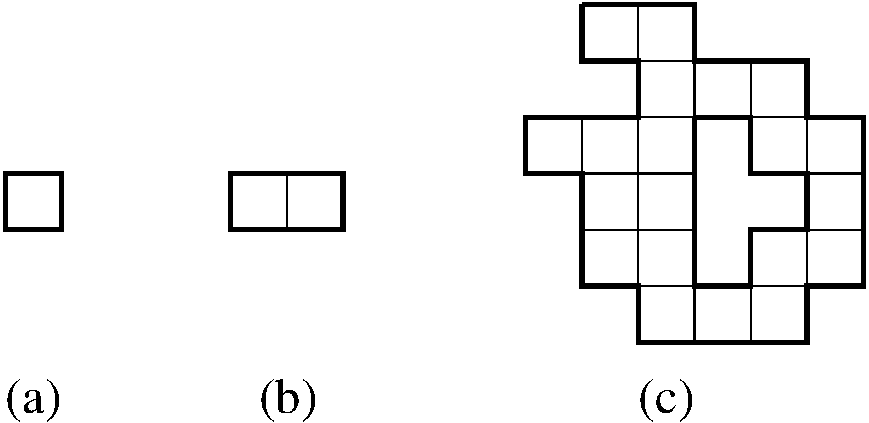
\includegraphics[width=4in]{figures/f98ps2}
\caption{Some shapes that Theory Hippotamus created.} \label{fig:squares}
\end{figure}

\begin{solution}

The proof is by induction.  Let $P(n)$ be the proposition that the
periphery length is even after $n$ squares are placed.  In the base
case, $P(1)$ is true because the periphery of a single square has
length 4, which is even.

In the inductive step, assume that the periphery length is even after
$n$ squares are placed to prove that the periphery length is even
after $n+1$ squares are placed.  The $(n+1)$-th square could share 1,
2, 3, or 4 edges with previously-placed squares.

\begin{itemize}

\item If the new square shares 1 edge with a previously placed square,
then this one edge is removed from the periphery, but three edges of
the new square are added to the periphery.  Overall, the periphery
length increases by two and thus remains even.

\item If the new square shares 2 edges with previously placed squares,
then these two edges are removed from the periphery, but two edges of
the new square are added.  The periphery length is unchanged and thus
remains even.

\item If the new square shares 3 edges, then these three edges are removed
from the periphery, but one edge is added.  The periphery length
decreases by two and remains even.

\item If the new square shares 4 edges, then these four edges are removed
from the periphery and none are added.  The periphery length decreases
by four and remains even.

\end{itemize}

In all cases, the length of the periphery remains even.  Therefore,
for all $n \geq 1$, $P(n)$ implies $P(n+1)$ and the claim is proved by
induction.

\end{solution}

\end{problem}
